\section{Joggle Design}
\label{sec:design}

\subsection{System Model}
\label{sec:system-model}

Joggle represents programs and compiler extensions with the same typed graph
substrate. A \emph{subject mod} contains the program being inspected or
changed, whereas an \emph{extension mod} contributes compiler functions. Both
are ordinary mods: they use the same graph representation, type system,
dependency rules, and loader. The distinction describes their role in one
invocation, not two different runtime objects.

The graph owned by a mod is
\[
  G = (F, B, O, V, A),
\]
where $F$, $B$, $O$, and $V$ are functions, blocks, operations, and values, and
$A$ denotes attributes attached to these entities. Blocks order operations,
operations consume and produce values, and maintained def--use edges connect
each value to its users. Operator sets, input formats, and artifacts enter
through extension mods.

An environment $E$ loads the mods named by a program, resolves typed calls,
binds source or native implementations, and owns evaluator state. One
compiler-function call has the form
\[
  E \vdash f(M, a) \Downarrow (r, D, W).
\]
Here, $M$ is the subject mod and $a$ contains explicit arguments. The call
returns $r$, records the observed graph state $D$, and publishes graph effects
$W$. Read-only calls have $W=\varnothing$. Mutating calls produce $W$ only
after the resulting graph passes verification.

Joggle calls this representation progressive because each successful compiler
function publishes another verified mod over the same entity model. A stage may
retain semantic operations while introducing lower-level helpers, and a later
stage may replace definitions it owns. Typed refinements express progress
within one graph model, and every published state remains inspectable.

The rest of the design follows the three requirements from
Section~\ref{sec:requirements}. Section~\ref{sec:compiler-functions} realizes
R1 with typed compiler functions. Section~\ref{sec:mods} realizes R2 with
mod-scoped composition. Sections~\ref{sec:incremental}
and~\ref{sec:graph-runtime} realize R3 through observed dependencies and the
graph runtime that validates them.

\subsection{Compiler Functions}
\label{sec:compiler-functions}

Joggle's metaprogramming interface is the typed compiler function. Operator
semantics, analyses, transformations, representation conversion, and artifact
generation use this single programmable surface for definition and invocation.

A compiler function accepts graph handles and ordinary values:
\[
  f : (H_1, \ldots, H_n, A_1, \ldots, A_m) \rightarrow R.
\]
Each $H_i$ is a \texttt{Mod}, \texttt{Fn}, \texttt{Blk}, \texttt{Op}, or
\texttt{Val} handle. Each $A_i$ is a configuration or structural value, such
as an integer, type, list, dictionary, or \texttt{Attr}. The result $R$ may
itself be a handle, an ordinary value, structured data, text, or bytes. Handles
retain graph ownership and lifetime; ordinary values remain independent of
graph storage.

A common operator extension illustrates these roles in
Figure~\ref{fig:operator-extension}. A convolution, bias addition, and
activation form a fusible subgraph. One mod owns the fused
operator's semantic contract together with typed functions for legality
analysis, fusion, target conversion, and artifact generation. The functions
exchange graph handles and owned values through the interface above; each role
retains its own effect contract.

\begin{figure}[t]
  \centering
  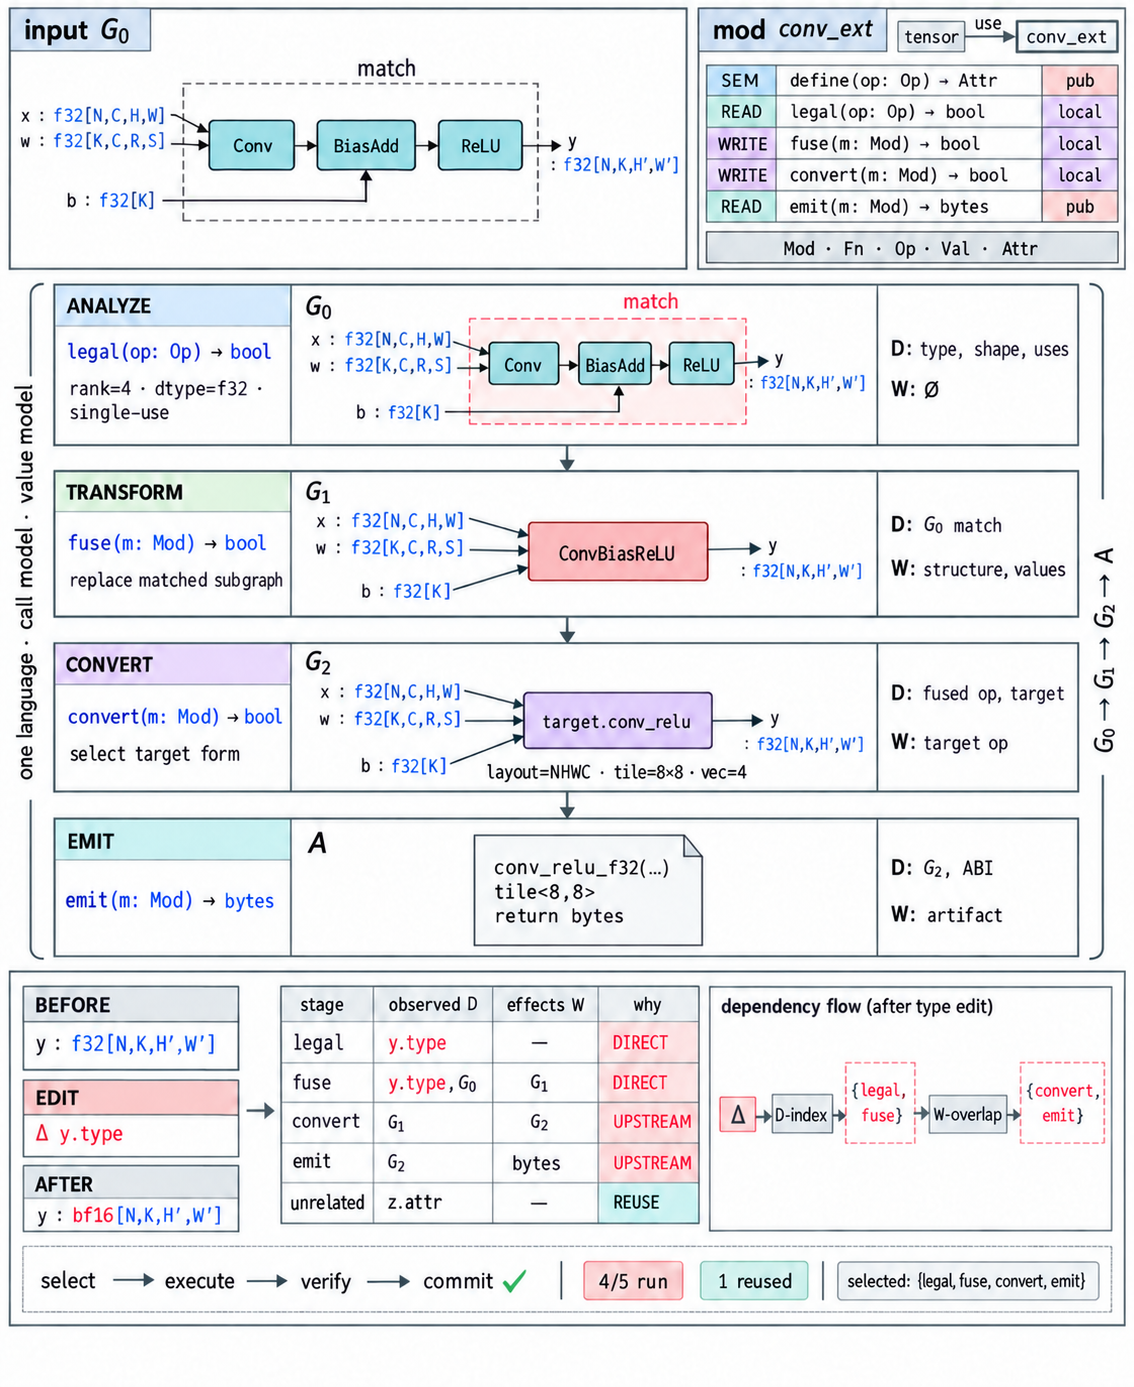
\includegraphics[width=\columnwidth]{figures/figure-03-operator-extension.png}
  \caption{One operator extension in Joggle. Five compiler roles share typed
  calls; recorded observations and effects select work after a local edit.}
  \Description{A typed convolution, bias, and activation graph is analyzed,
  fused, converted to a target operation, and emitted by five functions in one
  mod. The graph progresses through three verified states to an artifact. A
  type edit directly selects legality and fusion, propagates through conversion
  and emission, reuses an unrelated analysis, and commits transactionally.}
  \label{fig:operator-extension}
\end{figure}

Joggle resolves a call from its qualified name, visible mods, explicit generic
arguments, parameter types, and result context. The selected implementation may
be a source body, an intrinsic, or a native binding. Caller syntax and the
evaluator's result boundary remain identical across these implementations.

Uniform calls retain distinct effect contracts. A query evaluates against a
read-only mod and returns an \texttt{Attr}. A run applies one or more mutating
functions within a transaction. An artifact call evaluates read-only over a
prepared graph and returns text or bytes. Thus, \texttt{query}, \texttt{run},
and \texttt{emit} share resolution and evaluation while preserving different
publication rules. Read-only execution rejects mutation, and a run publishes
only a verified graph.

Compiler functions also compose through ordinary calls. A fusion function can
invoke its legality analysis, and a conversion can query the fused operator's
semantic contract. These calls remain visible to type checking, diagnostics,
and dependency capture. The typed call graph therefore defines composition
directly.

This function model unifies how compiler behavior is declared, resolved, and
invoked. Mods then supply the namespace, visibility, and dependency boundaries
that organize these functions.

\subsection{Mods}
\label{sec:mods}

A mod is Joggle's unit of ownership and composition. We model it as
\[
  \mathcal{M} = (n, U, F_{\mathrm{pub}}, F_{\mathrm{local}}, G, N).
\]
where $n$ is the mod name and $U$ is its declared \texttt{use} set.
$F_{\mathrm{pub}}$ and $F_{\mathrm{local}}$ are its public and local
functions, $G$ is its graph, and $N$ contains optional native bindings. The
loaded object is the semantic boundary; its on-disk package is the distribution
form.

The \texttt{use} declarations form a directed mod graph. Search roots determine
where a named mod can be found, while \texttt{use} edges select the dependencies
that participate in loading and resolution. Separating location from dependency
keeps neighboring installations outside the visible function set.

Loading validates the declared dependency closure before evaluation. The loader
rejects missing mods, cycles, declaration-name mismatches, duplicate public
signatures, unreadable fragments, and unresolved native bindings. It then loads
source fragments in deterministic order. For a fixed mod graph and search-root
order, this process yields a stable public function set.

Visibility keeps this public set small. A public function can be resolved by a
dependent mod, whereas a \texttt{local fn} remains inside its owner. Source
fragments may split a large implementation without creating new dependency or
lifecycle boundaries. A separate mod is appropriate when a capability needs an
independent public surface, dependency set, owner, or installation lifecycle.

Native code follows the same boundary. A body-less declaration names the typed
contract, and a native library owned by that mod supplies its implementation.
The binding is scoped to the owning mod and becomes available through the
declared dependency graph.

Lifecycle operations preserve the same closure. Installation stages a
candidate, loads and verifies its dependencies, and publishes it only after
validation succeeds. Upgrade additionally checks affected reverse dependencies.
A failed operation leaves the installed graph unchanged. These rules make the
mod the unit that evolves across installation and upgrade.

The mod graph is orthogonal to the containment structure inside a subject
program. Blocks and operations describe program structure; \texttt{use} edges
describe compiler capability. The former may change during transformation
without rewriting the latter. This separation lets one project compose
analysis, transformation, and artifact mods without embedding those ownership
decisions into its program IR.

Static mod dependencies state what a compiler extension may call. During
execution, the evaluator records which functions and
graph entities a call actually observes. Section~\ref{sec:incremental} uses this
second, dynamic dependency graph to avoid re-executing unaffected work.

\subsection{Incremental Evaluation}
\label{sec:incremental}

A local graph edit need not invalidate every compiler result. Joggle bases reuse
on observed state rather than on the subject mod's whole revision alone. For a
cached read-only call $c$, the evaluator stores
\[
  C_c = (K_c, r_c, D_c),
\]
where $K_c$ identifies the environment, store, function, and arguments; $r_c$
is the returned value; and $D_c$ contains the observations made while computing
it.

Observations follow the graph API used by the function. Reading one operation
records its identity, generation, and payload state. Reading one value also
records type, metadata, and def--use state. Traversing a function records the
relevant function revision or collection membership. Reading all operations,
the mod structure, or the \texttt{use} set records progressively broader state.
The evaluator therefore captures the narrowest observation that preserves the
semantics of each graph operation.

Range access records the structural revision together with only the returned
operations. A content edit outside the range therefore preserves the record,
whereas insertion, removal, or reordering invalidates its structural premise.

A cached query is reusable when its call key and every recorded observation
remain current:
\[
  \operatorname{Reusable}(c) = \operatorname{Same}(K_c) \land
  \bigwedge_{d \in D_c} \operatorname{Current}(d).
\]
On a hit, the evaluator returns $r_c$. On a miss, it evaluates the function in
read-only mode, captures a fresh $D_c$, and replaces the entry. The execution
report names the first invalid contract, such as an environment, structure,
function, operation, or value change. Generation checks distinguish an edited
entity from a new entity that later reuses the same slot.

Mutating pipelines require one further step. After a successful run, a reactive
schedule stores for each stage $s_i$ its call key $K_i$, observed inputs $D_i$,
and output scope $W_i$. The key names the environment, function, and arguments.
The output scope contains changed function identities and flags for structural
or mod-dependency changes. On the next run, a stage is selected when its key or
inputs are stale, or when an earlier selected stage may change something it
observed:
\[
  \begin{aligned}
    \operatorname{Selected}_i ={}&
      \neg \operatorname{Current}(K_i,D_i) \\
      &\lor \exists j<i:\ \operatorname{Selected}_j \land
      \operatorname{Overlap}(W_j,D_i).
  \end{aligned}
\]
The second term is an \emph{upstream} miss. The inputs recorded for $s_i$ may
still match at the start of a run, yet an earlier stage selected in the same run
can change them. Propagating recorded output scopes restricts downstream
selection to overlapping regions instead of forcing all later stages to execute.

\begin{algorithm}[t]
  \caption{Reactive stage selection and execution}
  \label{alg:reactive}
  \begin{algorithmic}[1]
    \State $dirty \gets \varnothing$; $selected \gets \varnothing$
    \For{each stage $s_i$ in schedule order}
      \State $miss \gets \operatorname{validate}(K_i,D_i)$
      \If{$miss=\varnothing \land \operatorname{overlap}(dirty,D_i)$}
        \State $miss \gets \mathrm{upstream}$
      \EndIf
      \If{$miss\neq\varnothing$}
        \State $selected \gets selected \cup \{s_i\}$
        \State $dirty \gets dirty \cup W_i$
      \EndIf
    \EndFor
    \State begin transaction
    \For{each $s_i\in selected$ in schedule order}
      \State execute $s_i$ and capture fresh $D_i,W_i$
    \EndFor
    \State verify and commit graph
    \State replace selected records and rebase retained records
    \State publish all records for the next run
  \end{algorithmic}
\end{algorithm}

Dependency records are published only after all selected stages execute and the
final graph verifies. Failure rolls back graph mutations and revision state; it
also discards the tentative records. Consequently, the next run cannot reuse
dependencies derived from an unpublished graph.

In Figure~\ref{fig:operator-extension}, a type edit directly invalidates the
legality and fusion stages that observed it. Because fusion may replace the
matched subgraph, conversion is selected by overlap with that potential
effect; artifact generation follows conversion for the same reason. An
analysis with disjoint observations retains its previous result.

Fine-grained observations reduce re-execution but add capture and validation
work. For $K$ stages, incremental latency is approximately
\[
  \begin{aligned}
    T_{\mathrm{select}}
      &= \sum_{i=1}^{K} T_{\mathrm{validate}}(K_i,D_i)
         + T_{\mathrm{propagate}}, \\
    T_{\mathrm{inc}}
      &= T_{\mathrm{select}}
         + \sum_{s_i \in \mathrm{Selected}} T_{\mathrm{eval}}(s_i) \\
      &\quad + T_{\mathrm{verify}}(G') + T_{\mathrm{commit}}.
  \end{aligned}
\]
Reuse is beneficial when this cost is lower than executing the omitted stages.
Broad graph APIs remain correct but record broad dependencies; narrow APIs can
preserve results across unrelated edits. External mutable state must enter
through typed arguments or an environment change before reuse. Native bindings
exchange scalar or byte attributes and do not receive graph entities, so
graph-dependent work remains in tracked compiler functions. These rules define
the state over which Joggle can validate reuse.

Incremental evaluation therefore depends on more than a result cache. It
requires stable entity identity, revisions that reflect every published edit,
and transactions that align graph state with dependency state. The graph
runtime provides these mechanisms.

\subsection{Graph Runtime}
\label{sec:graph-runtime}

Each mod owns a store with separate slot arrays for functions, blocks,
operations, and values. Public graph entities are small handles
\[
  h = (S, i, g),
\]
where $S$ identifies the store, $i$ selects a slot, and $g$ is that slot's
generation. A lookup succeeds only when the store matches and the slot is live
at generation $g$. Erasing an entity advances its generation, so a stale handle
cannot refer to a later entity that reuses the same slot.

The store maintains whole-mod, structural, and function revisions. Any
observable edit advances the whole revision. Membership, order, and topology
changes also advance the structural revision, while function-local changes
advance the owning function's revision. These counters serve as freshness
tokens. Their granularity lets a function-level
observation survive an unrelated edit elsewhere in the mod.

Graph relations are updated with the store. In particular, each value records
its users. Replacing a value can therefore walk the affected uses, update both
def--use lists, and touch the owning functions without scanning every operation.
Repeated affected-cone walks use epoch marks, avoiding a graph-sized bitmap
clear before each sparse traversal.

Mutations execute inside a transaction. Metadata edits journal the previous
leaf value. Structural edits acquire a store snapshot lazily, when the first
such edit occurs. After evaluation, the verifier checks ownership, liveness,
dominance, calls, block arguments, return types, and structured control flow.
The publication rule is
\[
  \operatorname{Publish}(f,G) =
  \begin{cases}
    (G', \mathrm{ok}) &
      \text{if } f:G \Downarrow G'
      \land \operatorname{Verify}(G'), \\
    (G, \mathrm{fail}) & \text{otherwise.}
  \end{cases}
\]
Verification therefore prevents a locally valid edit from exposing a globally
invalid graph. Success commits the graph and its revisions; failure restores
both.

The evaluator uses predecoded plans for checked compiler functions. A plan maps
parameters, block arguments, and operation results to dense slots; it
also records block targets, operation kinds, operand indices, and call-site
information. Its cache key is
\[
  \operatorname{PlanKey} =
  (S, \operatorname{id}(fn), \operatorname{generation}(fn),
   \operatorname{revision}(fn)).
\]
Changing a function body invalidates its plan, while calls to the same version
reuse decoding and slot layout. Stable call sites additionally cache overload
resolution under the current environment epoch and argument types. Reusable
register windows reduce per-call allocation.

These plans are an internal interpreted execution form. They remove repeated
decoding and slot-allocation setup while preserving the language's control
flow, failure propagation, and dynamic calls. A native implementation may
accelerate a specific typed function through the same mod-scoped binding and
graph API.

At the extension boundary, typed handles represent live graph identity and
\texttt{Attr} represents owned, serializable values. Dependency records,
execution plans, transaction journals, and counters remain private. This
boundary keeps runtime machinery out of the extension API while allowing
reports and profiles to evolve as structured data.

Together, stable handles, hierarchical revisions, transactional mutation, and
versioned execution plans make the higher-level design operational. Compiler
functions can manipulate live graph entities, mods can evolve independently,
and the evaluator can reuse work while preserving graph and dependency
publication boundaries.
